\documentclass[../ClassicThesis.tex]{subfiles}
\begin{document}

%************************************************
\chapter{Joint Computation / Klara}\label{ch:joints}
\newcommand{\TODO}[1]{\textcolor{red}{\\ \textbf{TODO:} #1 \\}}
%************************************************

% Use active Voice (we do….)
% Ein Gedanke pro Paragraph
% Terminologie anpassen über alle Arbeiten hinweg (was ist eine Plate für alle…)
% Jeder sollte eine kleine Related Work section haben
% Erklärungen zu warum dieser Algorithmus genutzt wurde und nicht ein anderer + limitations des gewählten Algorithmus
% Hübsche Bildchen zum anschaulichen Erklären!! (ebenfalls konsistent halten: gleich geformte labels etc.)

\section{Joint computation}
A lasercutted object needs connectors if it consists of multiple parts. Those can be elements like screws, nails and glue. Or the plates already come along with connectors. Those can be for example fingerjoints which, when well calibrated, do not need any external material to hold together. \\
Whenever possible we want to provide connections like that because a user needs less effort when components work directly out of the lasercutter. This is why we provide three types of joints which are added to the determined plates.\\
The previous \hyperref[ch:graph]{plate graph step} provides all edges that need to receive joints, the angle of each edge and the line along which each plate receives the joints.

\section{building joints}
The general procedure of creating joints consists of three steps: First we calculate how many female and male joints fit onto the intersection. Then the retrieved joints are placed at the intersection line and the shapes are merged to result in the original plate with joints.
\subsubsection*{Building the joints for a specific intersection line}
First we find out how many joints, males and females, fit along the length of the line.
Since all joint types have equal widths for female and male joints we divide the length of the line by the width of a joint.\\
\*\\
% \paragraph{adjustJointWidth}
But the result from this calculation has to be rounded because the number of joints just found do not necessarily work out evenly with the length of the line. This yields us a whole number which defines how many joints we need to create. Then we adjust the width so that the joints will be evenly spread without leaving space on either end of the line.\\
Now that we know how the joints will look like and how many we need it is time to find out how to distribute them.\\
In order to always create a well defined female and male part we place a thick joint in the center of the line if there are an even number of joints to be distributed, see fig. \ref{fig:evenOddCount}.\\
\begin{figure}[!ht]
\centering
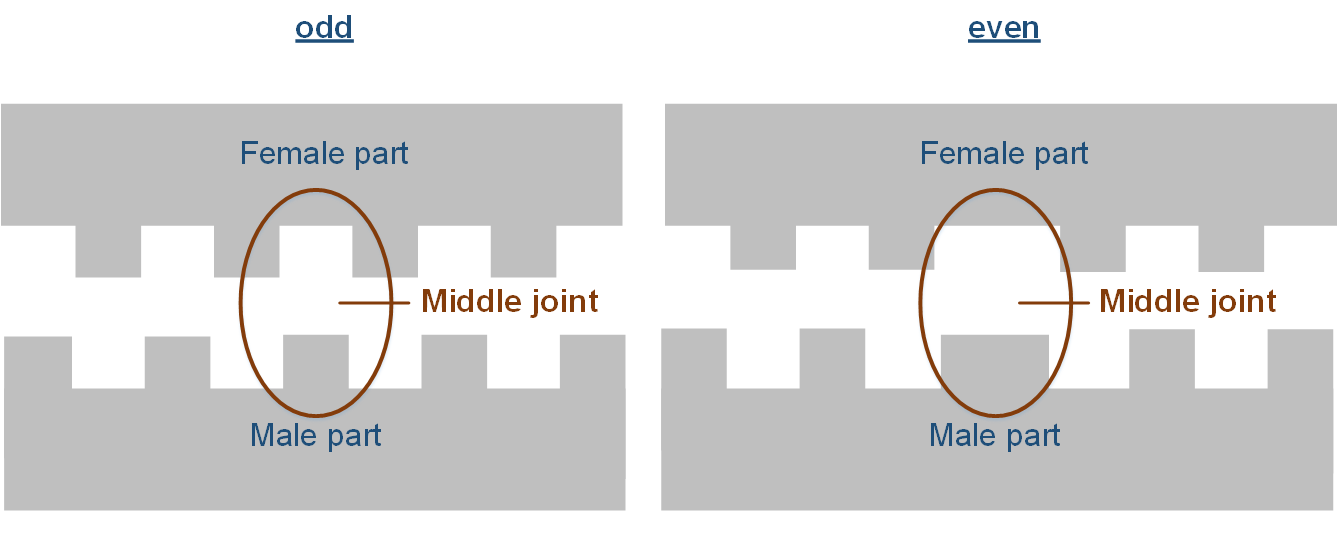
\includegraphics[width=\columnwidth]{Images/10-joints-evenOddJointsCount.png}
\caption{Distribution of joints depending on the number of joints. An even number results in a thick inner joint.}
\label{fig:evenOddCount}
\end{figure}

% \paragraph{computeMaleJointsPerSide} %number only
On both sides of the middle joint will be an equal number of male joints. How many depends on the jointCount. An even jointCount means 2 joints less and odd means one joint less on the sides because the middle joint will be created seperately. Since the jointCount specifies the number of all joints, male and female we have to divide by two to get the number of male joints only and then divide by two once more to achieve the seperation into the two sides.\\
maleJointsPerSide = 
\begin{cases} 
(jointCount - 2) / 4, & jointCount $ \% 2 == 0 $ \\ 
(jointCount - 1) / 4, & jointCount $ \% 2 == 1 $
\end{cases}\\
\*\\
% \paragraph{buildJointsForEven / Odd count}
Finally, we can start placing the middle joint and distributing as many joints as just calculated on either side of it evenly with leaving enough space in between the joints for a female one to fit in as can be seen in figure \ref{fig:spreadedJoints}.
\begin{figure}[!ht]
\centering
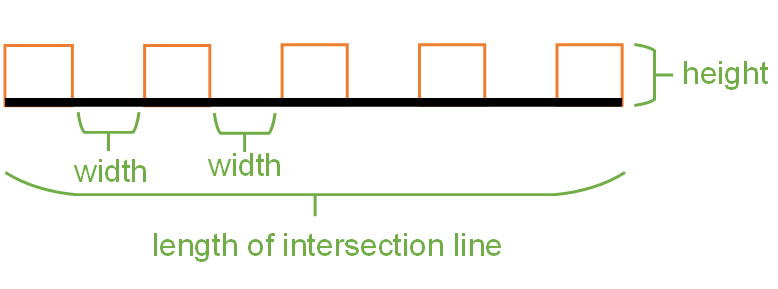
\includegraphics[width=\columnwidth]{Images/10-joints-spreadedJoints.png}
\caption{The joints are spreaded evenly along the line leaving space of a joint with in between for the other plates joints to fit in.}
\label{fig:spreadedJoints}
\end{figure}
% \paragraph{computeFemaleJointsPerSide} %number only
The computation for the number of female joints on one side of the middle joint is very similar to the previous computation for male joints. Only that the middle joints do not have to be subtracted.\\
femaleJointsPerSide = 
\begin{cases} 
(jointCount) / 4, & jointCount $ \% 2 == 0 $ \\ 
(jointCount + 1) / 4, & jointCount $ \% 2 == 1 $
\end{cases}\\
\*\\
% \paragraph{create Females for fingerjoint type}
When creating \emph{fingerjoints} the female joints are the exact negative of the male joints. Therefore we do not create these joints one by one. Instead we retrieve the boundingbox of the male joints along the length of the intersection line and calculate the difference of this rectangle and the male joints. The result are the female joints.\\
\*\\
% \paragraph{create Females for jimjoints/dovetail joints}
In the case of \emph{dovetail}- and \emph{jim-joints} we have to create the female joints by placing each single joint along the intersection line.\\
This is achieved by distributing them in the same way as the male joints are evenly spread. Except that for the females we leave the space for the middle joint empty.\\
Finally, we have created female and male joints which are aligned along a line with the length of the intersection.
    
\subsubsection*{Placing the joints at the correct edge of the plate}
This step moves the joints to the correct position in space. 
% \paragraph{line and shape into XY}\\
\*\\
To do shape union functions we need to move the shape of the plate and the intersectionline into the xy-plane.
\*\\
% \paragraph{bounding box of joints, center of bounding box}
The joints which already lie in the xy-plane are rotated and translated onto the intersectionline.\\
\*\\
% \paragraph{make sure joints are placed at line but outside of shape}
To make sure that the joints will be appended to the plates we test if the transformed joints lie inside the plate. If so they are moved towards the outside of the plate.
            
\subsubsection*{Merging the joints with the plate}
The last step unions the now aligned shapes of the joints and plates and rotates them to the correct position in space where the plate belongs to within the model.


\section{Different Fingerjoint types}
We support three types of joints. Each have benefits when used for specific material. For example acylic is not flexible which means it is very sturdy, but bendable when heated. \\
We allow the user to choose the type of material which then affects the choice of joints in the converted model.

\subsubsection{Fingerjoint template}

\begin{figure}[!ht]
\centering
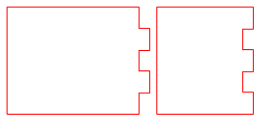
\includegraphics[width=.5\columnwidth]{Images/fingerjoints.png}
\caption{Path which a lasercutter has to follow to cut our plates with fingerjoints.}
\label{fig:fingerjoints}
\end{figure}


%\paragraph{How these joints look like}
Fingerjoints, see fig. \ref{fig:fingerjoints}, only consist of 90 degrees angles. The female joints are the exact inverse of the male joints. This means that the joints can slide directly into each other. 

But that only works when the sizes are measured correctly so that they create a tight fit. Otherwise plates connected by fingerjoints do not fit into each other at all or fall apart and have to be glued. 
%\paragraph{How these joints work, and for what material}
When using fingerjoints one typically has 90 degree angled plates because it is the easiest way to connect them. Other angles can be created but it is hard to know when the plates form the exact angle that is wanted unless the plates are part of a construction which gives them no other choice than to form the given angle.
\TODO{Maybe show this in a picture? Boat vs only two plates, where the angle cannot be determined without the other plates}
Regarding the material fingerjoints are useless when flexible materials are connected with it. The problem is that a tight fit cannot be created in most cases. Also very thin material is not working well since fingerjoints hold up due to the friction of one plate to the other. The fewer material the less friction.\\
We usually use fingerjoints for acrylic and wood.


\subsubsection{JimJoint template}


JimJoints, see fig. \ref{fig:jimJoints}, are named after Jim McCann who thankfully showed us the design for these connections.
%\paragraph{How these joints look like}
The male and female joints are the same but they grow wider with its height.

\begin{figure}[!ht]
\centering
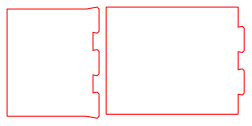
\includegraphics[width=.5\columnwidth]{Images/jimjoints.png}
\caption{Path which a lasercutter has to follow to cut our plates with JimJoints.}
\label{fig:jimJoints}
\end{figure}

This means these joints cannot slide into each other but they rather snap together. This means once they are connected they cannot be taken apart just by pulling on the plates. 

%\paragraph{How these joints work, and for what material}
In order for the snapping to work the material has to be flexible or very thin. Jim McCann already used it for foam. We now use it especially for paper because this material would be too thin for creating enough friction for fingerjoints to work.

\subsubsection{Dovetail template}
\begin{figure}[!ht]
\centering
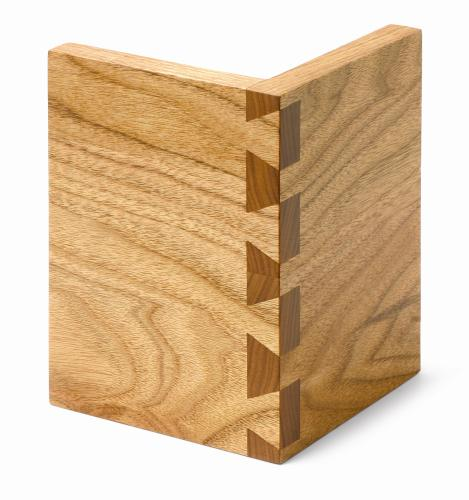
\includegraphics[width=.5\columnwidth]{Images/dovetails-wood.jpg}
\caption{Original dovetails created with a mill in wooden plates.}
\label{fig:realDovetailJoints}
\end{figure}

\begin{figure}[!ht]
\centering
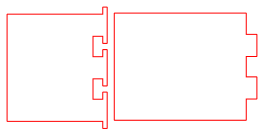
\includegraphics[width=.5\columnwidth]{Images/schwalbe.png}
\caption{Path which a lasercutter has to follow to cut our plates with dovetails.}
\label{fig:dovetailJoints}
\end{figure}
    
    Typically a dovetail joint is used in woodwork, see fig. \ref{fig:realDovetailJoints}. It helps to ensure that when there is a pulling force on both wooden plates that the joints all hold onto the other plate.\\
    But in order to create the female joints the wood needs to be cut in an angle. This is not possible without inadequately high time and power consumption. See the upcoming section \hyperref[futureWork]{Future Work} for information on how to lasercut the female part of a dovetail.\\
    Instead, we developed a joint type, see fig. \ref{fig:dovetailJoints}, very similar to the original dovetail. This can be easily cut with a lasercutter.
    %\paragraph{How these joints look like}
    The males and females are alot like typical fingerjoints. But the females have an additional part which will fixate the other plate from one direction.\\
    %\paragraph{How these joints work, and for what material}
    These joints now withstand a force pulling away the plate with the female joints. It works with any material with at least around one millimeter of thickness when the material is not very flexible.

\subsection{Adjusting fingerjoints length when plates are angled}
    % \paragraph{adjustJointHeight}
    Not only the width has to be adjusted but also the height needs to be adapted to the plates connection. Depending on the angle of the plates the joints need to be longer or shorter accordingly.\\
    This problem can be solved by using trigonometry within the geometry of the overlap of the plates.\\
    If the plates overlap they create a parallelogram, see fig. \ref{fig:newJointHeight}. The length of the long diagonal \emph{d} is the key to finding the appropriate length for the joints.
    \begin{figure}[!ht]
    \centering
    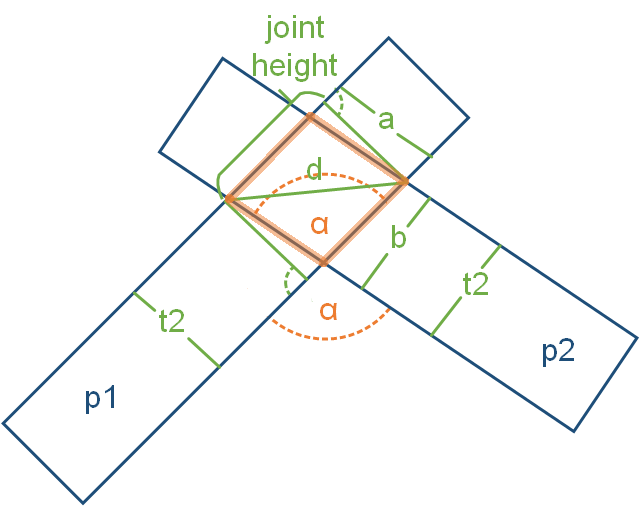
\includegraphics[width=0.5\columnwidth]{Images/06-2-joints-newJointHeight.png}
    \caption{The parallelogram spanned by the overlap of the plates allows us to find the appropriate height for a joint.}
    \label{fig:newJointHeight}
    \end{figure}
    
    We have already calculated the angle between the plates earlier and can now use it to find the lengths of the sides \emph{a} and \emph{b} of the parallelogram by the help of trigonometry:\\
    Thickness of plate $p_1$: $t_1$\\
    Thickness of plate $p_2$: $t_2$
    $$ a = t_1 / sin(180^{\circ} - \alpha)$$
    $$ b = t_2 / sin(180^{\circ} - \alpha)$$
    
    This helps us to calculate the length of the diagonal \emph{d}:
    $$ d = \sqrt{a^2 + b^2 - 2ab * cos(\alpha)}$$
    Finally, the triangle with the sides \emph{d, a, b} which helps us retrieve the height \emph{h} for the fingerjoints can be constructed. 
    
    $$ h = \sqrt{d^2 - a^2} $$
    
    Finally, this height can be applied to all joints of the current intersection line. This achieves that, when cut, the joints slide into each other, allowing to create the wanted angle.
    

\section{Alternative solutions}\label{alternativeSolution}

% \subsection{Wrong fingerjoint height adjustment}
% Firstly, the angle can be projected onto values between $0^\circ$ and $90^\circ$. Then the cosine function returns a number between 0 and 1 for the angle. The thickness of the plate is divided by this number to achieve a height that fits the angle and the thickness of the plates. 

\subsection{Dustin Beyers\citeauthor{master-thesis} approach to angles}
According to the master thesis on platener \cite{master-thesis} connections of plates can be seperated into four different angle types, see fig. \ref{fig:dustinsAngles}. This is based on the assumption that plates always overlap with an edge which is not the case as we found out.
He computed different angle types. They are quite crappy because he assumed that plates would only meet at edges. But plates can lie in one another.
\begin{figure}[!ht]
    \centering
    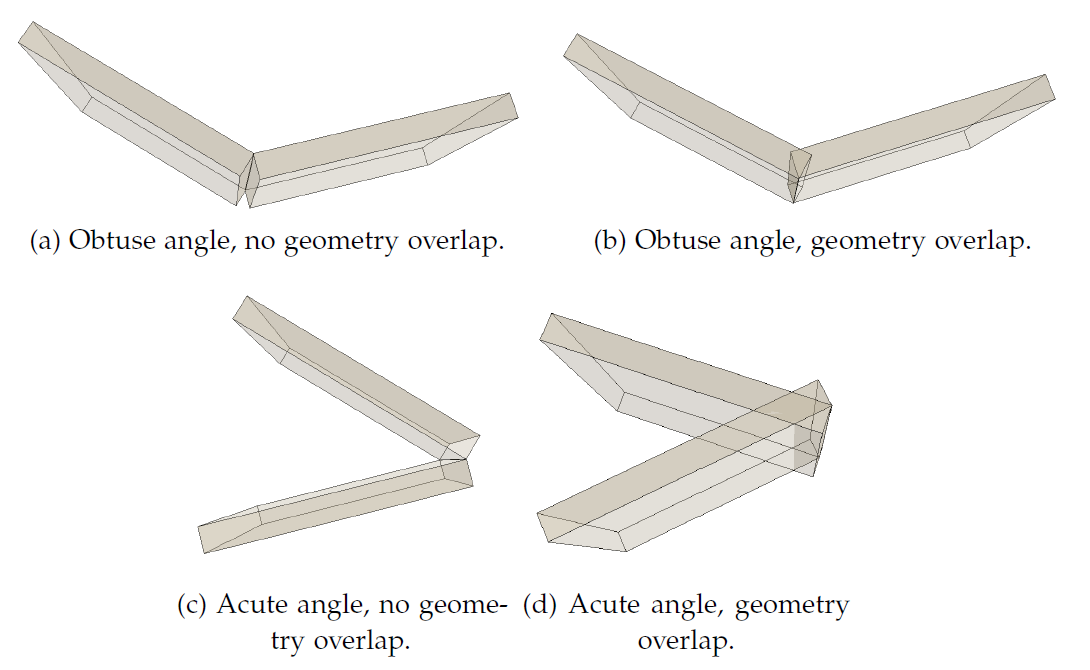
\includegraphics[width=1\columnwidth]{Images/06-1-graph-dustinsAngleImage.png}
    \caption{Figure from the thesis \cite{master-thesis} showing the different angle types.}
    \label{fig:dustinsAngles}
\end{figure}
Therefore we do not use those angle type but we clip both plates with their four intersection lines. \\
Then due to angle and trigonometry etc. we can calculate the correct length for the joints which connects the plates again.

\section{Future work}\label{futureWork}
\subsection{Additional joint types}
In figure \ref{fig:additionalJoints} we show different types of joints which could be added to our repertoire.
\begin{figure}
    \centering
\begin{subfigure}[b]{0.45\textwidth}
    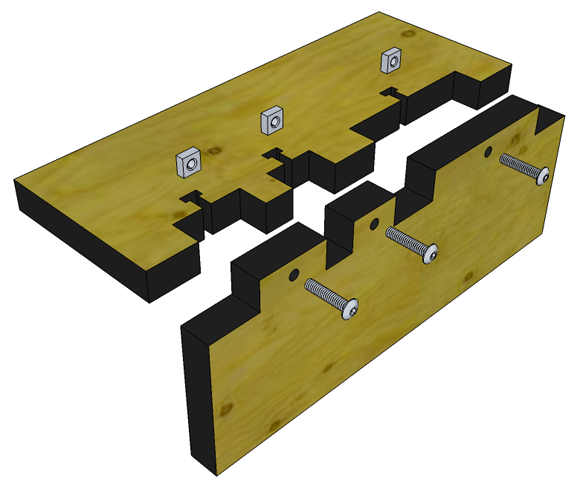
\includegraphics[width=\textwidth]{Images/pettis-joints.png}
    \caption{Pettis joint: fingerjoints with screws for more stability. Only 90$^\circ$ angles can be achieved.}
    \end{subfigure}
    ~
    \begin{subfigure}[b]{0.45\textwidth}
    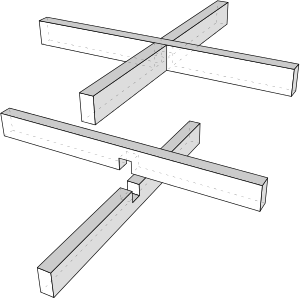
\includegraphics[width=\textwidth]{Images/HalvedJoint.png}
    \caption{Halved joint: slot joinery technique for plates which have an intersection through its middle.}
    \end{subfigure}
    
    \begin{subfigure}[b]{0.45\textwidth}
    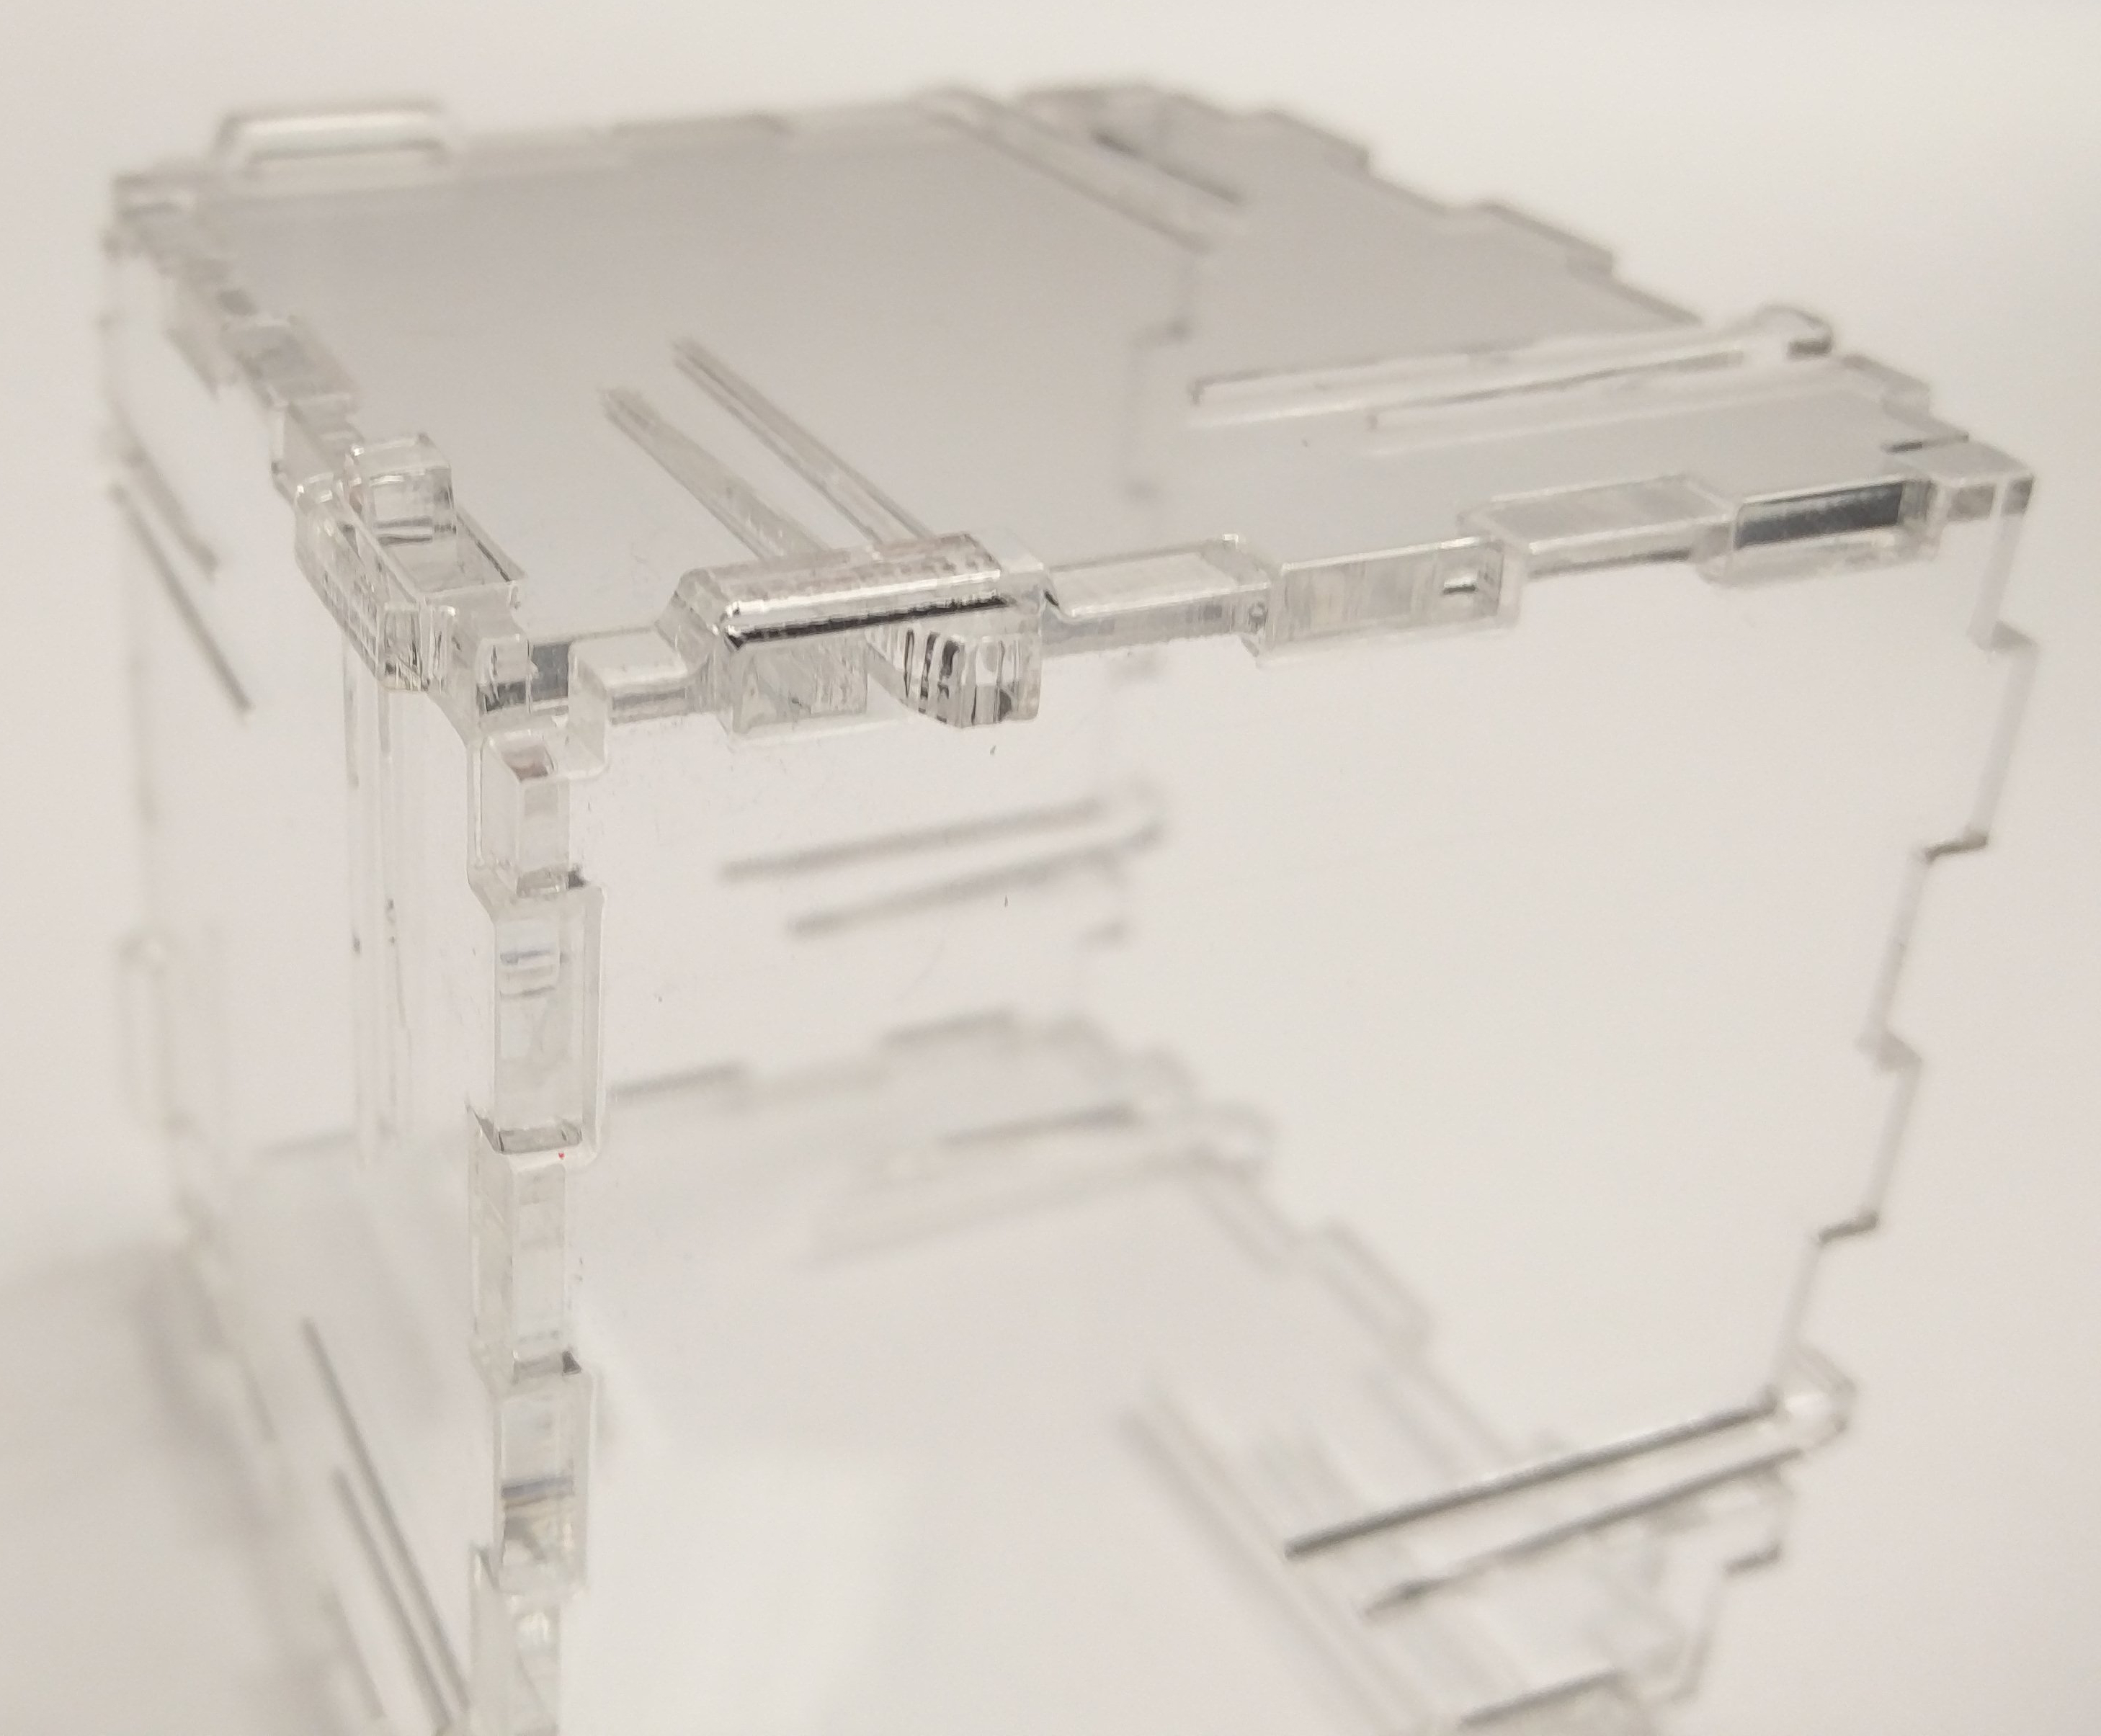
\includegraphics[width=\textwidth]{Images/snapfit.jpg}
    \caption{Snap fit: Using a Spring to snap into place. Holds tight, but takes up alot of space on the plate.}
    \end{subfigure}
    ~
    \begin{subfigure}[b]{0.45\textwidth}
    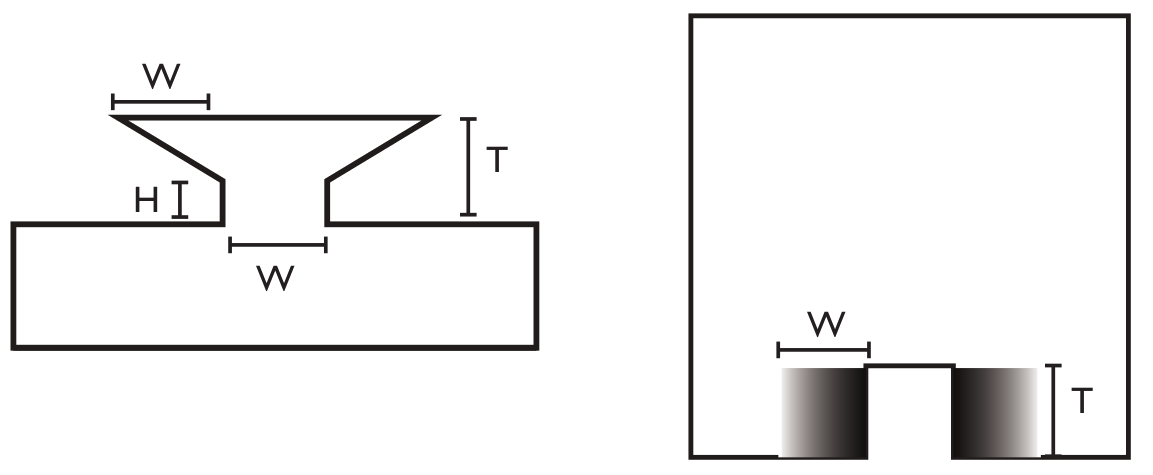
\includegraphics[width=\textwidth]{Images/06-2-joints-schwalbeMitLaser.png}
    \caption{Real dovetail: Using in a gradient \cite{lasercutLikeABoss} from white to black allows to cut different depths and achieve an angle.}
    \end{subfigure}
    \caption{Additional possibilites for connecting plates.}
    \label{fig:additionalJoints}
\end{figure}

\subsubsection{Joints should not stick out over the end of the intersection}
Currently, when using JimJoints or dovetails they might overlap the end of the line because the width value which is used for spreading the joints does not represent the with of the joint at its heighest point. This is because JimJoints and the females of the dovetails grow wider apart with its height.\\
In order to solve this the joint number should be calculated based on a joints maximum width, but they still have to be spread based on the minimum width.

\end{document}